\section{Cloud-based Burst Buffer System}
\label{sec:architecture}
% \kento{This section need to be totally reorganized. But please resolve my
% comments first}
% \kento{In this section, we need to describe information, which should be
% written in ``Users' manual'', not ``Developers' document''}
To validate the effectiveness of our cloud-based burst buffer system.
We design and implement a prototype of the system. In this section, we describe
the design.
%\begin
\subsection{Overview}
\kento{
\begin{itemize}
  \item Describe overview (compute nodes, burst buffer nodes, storage) in
  the Figure 4.
  \item Describe each role of compute nodes, burst buffer nodes, and
  stoarge
  \item What is the difference to conventional burst buffers 
\end{itemize}
}
% An overview of I/O burst buffer architecture is described in this section.
% As we mentioned in the previous section, our model takes advantage of high
% throughput inside a system, and use buffer queue system in order to increase
% throughput between two systems.
% %Two kinds of buffer are used in our I/O burst buffer architecture, the first one is in client computing node, first buffer user I/O in the same node, another one is in I/O buffer nodes.
% The main idea is that some of computing nodes serve as a I/O buffer nodes in
% each system, for write I/O data, if buffer queue in I/O buffer nodes is not
% full, data can first be buffered in buffer queue in the same system, and then client can finish write operation without waiting data be finally transferred to storage system.
% Actually, since many jobs use multiple nodes work together and the output of some nodes can be the
% input of the others, so for most cases, output data will still be buffered in
% buffer queue until the whole job finished.
% As for reading, if that file is stored in the buffer queue, compute nodes can
% read from I/O nodes through interconnection network.
% In other cases (buffer queue is full when issue a write request or requested
% file is not stored in buffer queue when issue a read request we call it cache
% miss), a read from or write back operation described below will be executed.

\begin{figure}[tb]
	\centering
	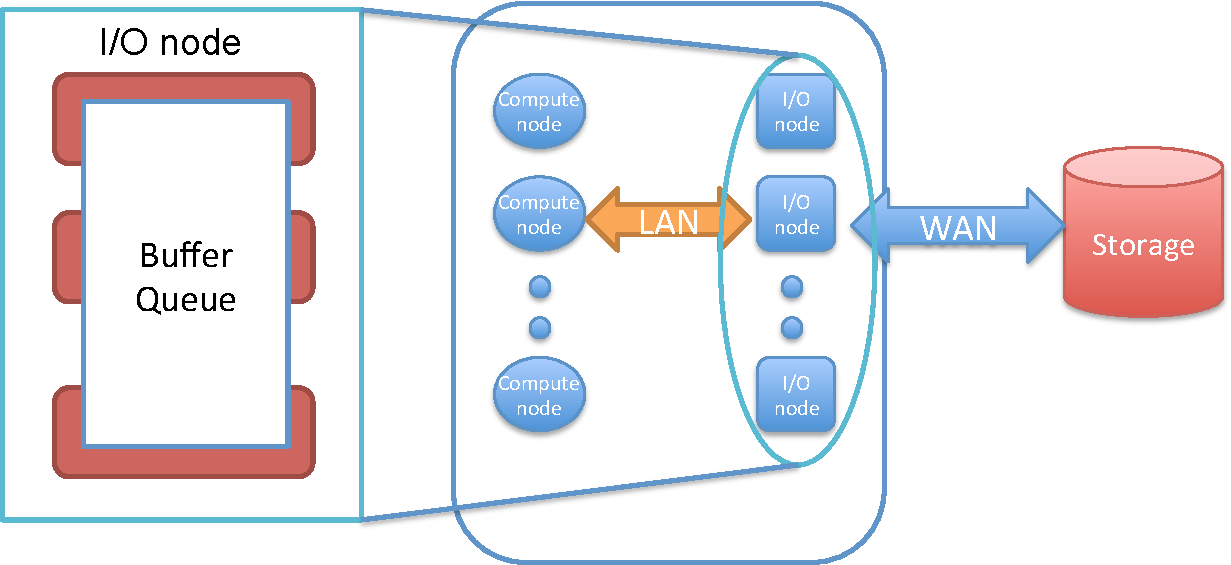
\includegraphics[width=8cm]{img/architecture_overview}
	\caption{overall illustrate of I/O Burst Buffer Architecture}
	\label{architecture:overview}
\end{figure}

Figure \ref{architecture:overview} shows a design overview of our cloud-based
burst buffer system, which consist of \emph{compute nodes}, \emph{burst buffers}
and a \emph{shared cloud storage}. \emph{Compute nodes} are nodes on which
applications run. \emph{Burst buffers} are provided by the same instances
as \emph{compute nodes}. Unlike \emph{compute nodes}, The instances
of the \emph{burst buffers} provide remote memory buffers for data caching.
When the applications read or write data, the I/O operations are handled via
\emph{burst buffers}.  The \emph{shared cloud storage} is persistent shared storage such as Amazon S3.
Because the applications read or write all data via the burst buffers, the
the caching operations under burst buffers is agnostic to the applications.
Hence, the applications can benefit from the two-level of storage hierarchy
without knowing the underlying operations.
 
An overview of I/O burst buffer architecture is described in this section.
As we mentioned in the previous section, our model takes advantage of high
throughput inside a system, and use buffer queue system in order to increase
throughput between two systems.
%Two kinds of buffer are used in our I/O burst buffer architecture, the first one is in client computing node, first buffer user I/O in the same node, another one is in I/O buffer nodes.
The main idea is that some of computing nodes serve as a I/O buffer nodes in
each system, for write I/O data, if buffer queue in I/O buffer nodes is not
full, data can first be buffered in buffer queue in the same system, and then
client can finish write operation without waiting data be finally transferred
to storage system.
Actually, since many jobs use multiple nodes work together and the output of
some nodes can be the input of the others, so for most cases, output data will
still be buffered in buffer queue until the whole job finished.
As for reading, if that file is stored in the buffer queue, compute nodes can
read from I/O nodes through interconnection network.
In other cases (buffer queue is full when issue a write request or requested
file is not stored in buffer queue when issue a read request we call it cache
miss), a read from or write back operation described below will be executed.

\subsection{I/O operations}
\kento{
\begin{itemize}
  \item How burst buffer start ?
  \item Mention the current prototype uses main memory. Why ?
  \item How the write operations works (e.g. chaching) ? and Why write
  performance is improved for applications ?
  \begin{itemize}
  	\item If the buffers are not full, \ldots
  	\item If the buffer are full, \ldots
  \end{itemize}
  \item How the read operation works (e.g. caching) ? and Why read performance
  is improved for applications?
  \begin{itemize}
  	\item If the data is in the buffers, \ldots
  	\item If the data is not in the buffers, \ldots
  \end{itemize}
  \item Any other things ?
  \item How burst buffers end ? What happens to data in the burst buffers ?
\end{itemize}
}



\subsection{Target Environment}
First, we introduce our target environment.
we target at common cloud environment like Amazon EC2, which compute node and data center are distributed geographically distributed.

\begin{itemize}
	\item All compute nodes are connected by large bandwidth and interconnection network, note network topology maybe different in each system, so topology is not specified here, interconnection network performance is measured by throughput.
	\item There is a shared storage for data sharing inside system, all compute nodes are connected
	with shared storage via Internet or other lower network, also the file system of shared storage is not specified and performance is measured by throughput.
\end{itemize}

\subsection{I/O Burst Buffer Architecture}


There are two kinds of nodes in our I/O burst buffer architecture: \emph{compute nodes} and \emph{I/O burst nodes}, compute nodes run user's application and I/O burst nodes.
Public clouds usually provide several type of instance for difference purpose, some are compute
optimized (like C3 instances provided by Amazon) provides a high compute performance, some are memory optimized (such as R3 instances in Amazon EC2) provide a huge amount of memory (up
to 244GB in R3 family), also memory size can be easily expanded by using solid storage driver (SSD)
as a swap device, usually such instances have SSD inside.

Fig.~\ref{architecture:overview} shows an overall illustrate of I/O burst buffer architecture.